%************************************************
\chapter{Resilience}\label{ch:resilience}
%************************************************
Topic 4: Write a brief introduction to Resilience in microservice architectures and to how Gatling load testing framework can be used for testing. Run load testing scenarios against the handed out containers and describe the effects of using patterns.
- run different load testing scenarios handed out
- hand-in generated reports and key metrics on BlackBoard 
- hand in exercise report
- run load-testing against your project architecture to see the effects

There are different categories of potential disruptions to system that create the need to implement the resilience in systems. In the figure \ref{ch:resilience} below the sources of disruptions is showed. 

\begin{figure}[bth]
	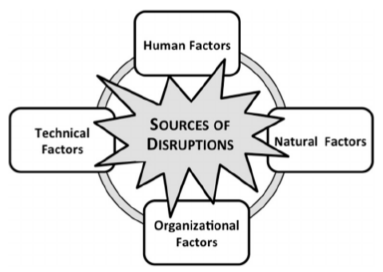
\includegraphics[width=0.7\linewidth]{gfx/resilience}
	\caption[routingtable]{Sources of disruptions} \label{fig:resilience}
\end{figure}   

\begin{itemize}
	\item Human Factor
	\begin{itemize}
		\item One of the common disruption is caused by human factors. The disruption in this case could be external attacks on the system, or just so simply as human using the system.  
	\end{itemize}
	\item Natural Factors
	\begin{itemize}
		\item A infrequent influence on damaging the system caused by natural disaster, such as floods and hurricane. 
	\end{itemize}
	\item Organizational factors
	\begin{itemize}
		\item Another difficulty to be considered about disruption the system is organizational factors, such as the worker strikes.   
	\end{itemize}
	\item Technical Factors
	\begin{itemize}
		\item Technical difficulty need also to be considered in the system. It is common that system component fails, and need to be either replaced or to be repaired.   
	\end{itemize}	
\end{itemize}

All the factors described above need to be considered in the system to avoid disruption. 

First of all the question is what is resilience? There are many definitions on that word depending on in what context it is used. In the sense of microservices the definition could sound: the power or ability to return to the original form, position, etc., after being bent, compressed, or stretched; elasticity.

Thus, from the definition above the resilient system should be able to cope with problem and at the same time be fast to recover. 

In the case of microservices the services are highly decoupled. By the isolation of microservices makes them independent from each other, so in the case of that one of them fails the other services do not stop working. By having the services decoupled in the system we get a lot of resilience into applications, thus they get ability to handle disruptions. 

   

This isolation of simple small services makes them independent from each other, so that when one fails the others don’t stop working.   

  





